% WR figure exported by sim_ui.py -- 2026-09-18 16:17:24
%
% Preamble (once, in your thesis):
%   \usepackage{pgfplots}
%   \pgfplotsset{compat=1.18}
%
% Use:
%   \begin{figure}[htbp]\centering
%     \input{wr_convergence}
%     \caption{...}\label{fig:...}
%   \end{figure}
%
% \input nests (unlike \include), so this works inside a chapter file the root
% already \includes. Pasting the body below inline works too -- the \definecolor
% lines may then be hoisted into the preamble and dropped from each figure.
%
% Series are thinned to ~2000 points each (min/max decimation, so spikes are
% preserved); edit _PGF_MAX_PTS in sim_ui.py for the full-resolution data.
%
% Run: coupling_mode=voltage-driven; precondition=on (optimized); interface_form=Thevenin (V source); use_t_floor=bare dt; interface_consistency=accumulated; N_field_windows=100; N_xyce_samples=1; xyce_integration_method=Backward-Euler (maxord=1)

\definecolor{C0}{HTML}{1F77B4}
\definecolor{C1}{HTML}{FF7F0E}
\definecolor{C2}{HTML}{2CA02C}
\definecolor{C3}{HTML}{D62728}

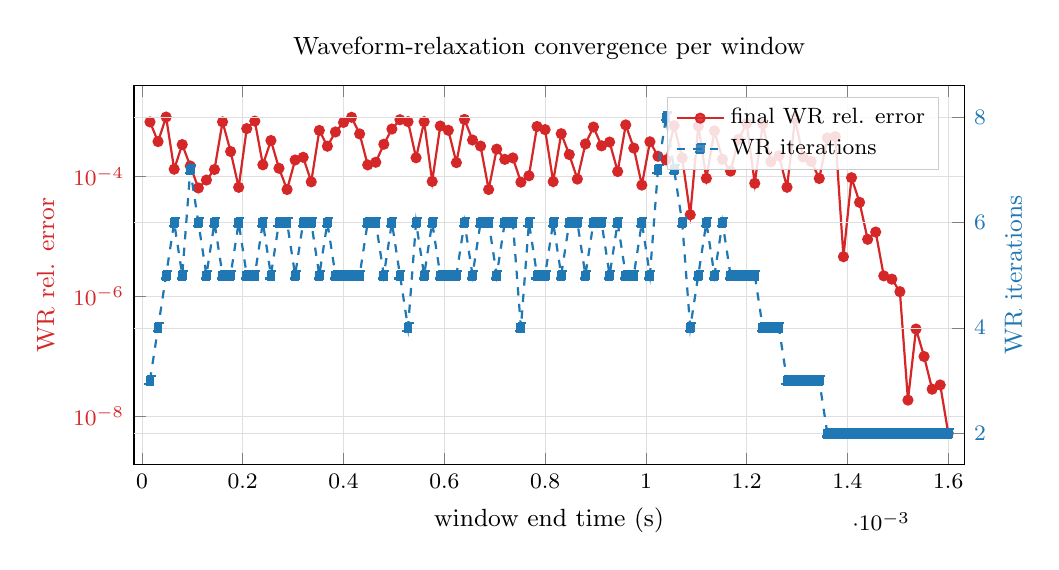
\begin{tikzpicture}
\begin{axis}[
  width=\linewidth,
  height=6.4cm,
  title={Waveform-relaxation convergence per window},
  xlabel={window end time (s)},
  ylabel={WR rel. error},
  grid=both,
  grid style={line width=.2pt, draw=gray!25},
  legend pos=north east,
  legend cell align=left,
  legend style={font=\footnotesize, fill=white, fill opacity=0.85, text opacity=1, draw=gray!40},
  tick label style={font=\footnotesize},
  label style={font=\small},
  title style={font=\small},
  scaled x ticks=true,
  xmin=-1.568e-05,
  xmax=0.00163168,
  ymode=log,
  axis y line*=left,
  ylabel style={color=C3},
  yticklabel style={color=C3}
]
  \addplot[color=C3, line width=0.8pt, mark=*, mark size=1.6pt] coordinates {
    (1.6e-05,0.0008189) (3.2e-05,0.000385) (4.8e-05,0.0009885) (6.4e-05,0.0001331) (8e-05,0.0003432) (9.6e-05,0.0001505)
    (0.000112,6.468e-05) (0.000128,8.769e-05) (0.000144,0.0001317) (0.00016,0.000822) (0.000176,0.0002627) (0.000192,6.637e-05)
    (0.000208,0.0006338) (0.000224,0.000845) (0.00024,0.0001574) (0.000256,0.0004007) (0.000272,0.0001378) (0.000288,6.103e-05)
    (0.000304,0.0001898) (0.00032,0.0002102) (0.000336,8.194e-05) (0.000352,0.0005907) (0.000368,0.0003222) (0.000384,0.0005568)
    (0.0004,0.0008037) (0.000416,0.0009788) (0.000432,0.0005172) (0.000448,0.0001571) (0.000464,0.0001738) (0.00048,0.0003475)
    (0.000496,0.000623) (0.000512,0.0008913) (0.000528,0.0008289) (0.000544,0.0002064) (0.00056,0.0008274) (0.000576,8.318e-05)
    (0.000592,0.0007006) (0.000608,0.0005939) (0.000624,0.0001715) (0.00064,0.0009022) (0.000656,0.0004084) (0.000672,0.0003238)
    (0.000688,6.101e-05) (0.000704,0.0002879) (0.00072,0.0001944) (0.000736,0.0002052) (0.000752,8.087e-05) (0.000768,0.0001034)
    (0.000784,0.0006875) (0.0008,0.0006094) (0.000816,8.264e-05) (0.000832,0.0005209) (0.000848,0.000234) (0.000864,9.103e-05)
    (0.00088,0.0003515) (0.000896,0.0006732) (0.000912,0.0003269) (0.000928,0.0003778) (0.000944,0.0001218) (0.00096,0.0007306)
    (0.000976,0.0002998) (0.000992,7.232e-05) (0.001008,0.0003818) (0.001024,0.0002189) (0.00104,0.0001902) (0.001056,0.00071)
    (0.001072,0.0002057) (0.001088,2.311e-05) (0.001104,0.0006986) (0.00112,9.362e-05) (0.001136,0.00058) (0.001152,0.0001948)
    (0.001168,0.0001238) (0.001184,0.0004199) (0.0012,0.0007739) (0.001216,7.735e-05) (0.001232,0.0007607) (0.001248,0.0001776)
    (0.001264,0.0002227) (0.00128,6.656e-05) (0.001296,0.0009168) (0.001312,0.0002136) (0.001328,0.0001796) (0.001344,9.32e-05)
    (0.00136,0.0004421) (0.001376,0.0004651) (0.001392,4.608e-06) (0.001408,9.591e-05) (0.001424,3.722e-05) (0.00144,8.997e-06)
    (0.001456,1.19e-05) (0.001472,2.209e-06) (0.001488,1.946e-06) (0.001504,1.203e-06) (0.00152,1.863e-08) (0.001536,2.859e-07)
    (0.001552,9.958e-08) (0.001568,2.833e-08) (0.001584,3.337e-08) (0.0016,5.222e-09)
  };
\end{axis}
\begin{axis}[
  width=\linewidth,
  height=6.4cm,
  title={},
  xlabel={},
  ylabel={WR iterations},
  grid=both,
  grid style={line width=.2pt, draw=gray!25},
  legend pos=north east,
  legend cell align=left,
  legend style={font=\footnotesize, fill=white, fill opacity=0.85, text opacity=1, draw=gray!40},
  tick label style={font=\footnotesize},
  label style={font=\small},
  title style={font=\small},
  scaled x ticks=true,
  xmin=-1.568e-05,
  xmax=0.00163168,
  axis y line*=right,
  axis x line=none,
  ylabel style={color=C0},
  yticklabel style={color=C0}
]
  \addlegendimage{color=C3, line width=0.8pt, mark=*, mark size=1.6pt}
  \addlegendentry{final WR rel. error}
  \addplot[color=C0, line width=0.8pt, dashed, mark=square*, mark size=1.6pt] coordinates {
    (1.6e-05,3) (3.2e-05,4) (4.8e-05,5) (6.4e-05,6) (8e-05,5) (9.6e-05,7)
    (0.000112,6) (0.000128,5) (0.000144,6) (0.00016,5) (0.000176,5) (0.000192,6)
    (0.000208,5) (0.000224,5) (0.00024,6) (0.000256,5) (0.000272,6) (0.000288,6)
    (0.000304,5) (0.00032,6) (0.000336,6) (0.000352,5) (0.000368,6) (0.000384,5)
    (0.0004,5) (0.000416,5) (0.000432,5) (0.000448,6) (0.000464,6) (0.00048,5)
    (0.000496,6) (0.000512,5) (0.000528,4) (0.000544,6) (0.00056,5) (0.000576,6)
    (0.000592,5) (0.000608,5) (0.000624,5) (0.00064,6) (0.000656,5) (0.000672,6)
    (0.000688,6) (0.000704,5) (0.00072,6) (0.000736,6) (0.000752,4) (0.000768,6)
    (0.000784,5) (0.0008,5) (0.000816,6) (0.000832,5) (0.000848,6) (0.000864,6)
    (0.00088,5) (0.000896,6) (0.000912,6) (0.000928,5) (0.000944,6) (0.00096,5)
    (0.000976,5) (0.000992,6) (0.001008,5) (0.001024,7) (0.00104,8) (0.001056,7)
    (0.001072,6) (0.001088,4) (0.001104,5) (0.00112,6) (0.001136,5) (0.001152,6)
    (0.001168,5) (0.001184,5) (0.0012,5) (0.001216,5) (0.001232,4) (0.001248,4)
    (0.001264,4) (0.00128,3) (0.001296,3) (0.001312,3) (0.001328,3) (0.001344,3)
    (0.00136,2) (0.001376,2) (0.001392,2) (0.001408,2) (0.001424,2) (0.00144,2)
    (0.001456,2) (0.001472,2) (0.001488,2) (0.001504,2) (0.00152,2) (0.001536,2)
    (0.001552,2) (0.001568,2) (0.001584,2) (0.0016,2)
  };
  \addlegendentry{WR iterations}
\end{axis}
\end{tikzpicture}
